\label{PVis-Guide}
\section{Introduction}

ParticleVis is an OpenGL visualization system designed to load and display particle simulation data.  It is purely a visualization tool, completely distinct from any simulation engine that may be used to generate particle data.  By loading in a file of particle state, the entire dataset can be visualized and explored in a fully realized three dimensional environment.

Notable features of ParticleVis include:
\begin{itemize}
	\item Real-time rendering of large-scale particle state data
	\item Export to PNG images or AVI movies
	\item Visualization of per-particle vector and scalar quantities
	\item Visualization of spatial vector fields
	\item Interactive color classification
	\item Fully configurable geometry parser for arbitrary particle shapes
	\item GLSL shader support for high-performance, high-fidelity visualization
\end{itemize}

\section{Basic Operation}

The data sources from which ParticleVis constructs visualizations are a series of simple file formats.  The fundamental data source is that of particle trajectories: a set of discrete objects with physical positions that are specified over time.

The ``statefiles'' that contain these fundamental trajectories must contain, at the minimum, blocks of particle positions.  In addition to position, the orientation of each particle and two vectors are acquired.  This pair of vectors describes the translational and angular velocities, in that order.

Since state files do not contain any description of the particle shape or appearance, an additional file that contains a geometric description of each particle is used to generate a more accurate visualization.  These particle descriptors contain XML-based markup that concisely specifies particle appearance.  An XML descriptor is paired with a single statefile or set of similar statefiles.  At runtime, an XML descriptor can be loaded at any time onto the currently loaded particles.

Other sources of data may also be integrated into the particle visualization.   The user may generate and load color map files, which specify arbitrary coloring of particles.  In the case of spherical paricles, surface map files allow specification of scalar quantities on the surface of each particle.  Free-form vector fields may also be placed into the visualization via the vector file format.  More detail about each of these datasources and the file formats associated with them is provided in subsequent sections.  

Minimal operation of the visualization application is accomplished by simply loading a statefile and using ParticleVis to play back and explore the data.  More accurate and visually pleasing visualization can  be obtained by loading an appropriate XML descriptor.  Additional data sources may then be added and integrated by parsing in additional filetypes.  In the ParticleVis application, the ``File'' menu contains all data acquisition commands.

Each file menu ``open'' or ``load'' entry corresponds to a filetype supported by ParticleVis.  Loading a statefile or XML descriptor will launch a file thread that will parse the input file in the background, allowing exploration of the partial dataset during loading.  To terminate the existing file loader threads, choose ``Terminate All File Processes'' from the file menu or press the comma key.  Color maps can also be loaded (with persisting and non-persisting color assignment).  For proper functionality, color maps should be imported only after the statefile has been fully loaded.  A command to load a bitmap texture image for use with polygonal particle rendering (``Use Textures'' under the View menu) is also present.  More detail about the various file formats and their syntax can be found in the file format guide.

Several miscellaneous commands reside in the file menu.  The first is ``Generate Benchmark Frame.''  This command will generate a single frame of particle state, with random positions.  The translational velocity will be set to the same value as the random position.  This feature is useful for testing features or evaluating the performance of the system.  Another file menu command is ``Report currently loaded data,'' which will briefly describe the currently loaded state and vector data.  The final miscellaneous command is ``Set all to Spheres,'' which will force all loaded particles to have a spherical geometry of specified radius.  The command can be convenient when the loaded data is simple and no descriptor is readily available.

\subsection{Camera Control}

The viewpoint in PVis is controlled primarily by mouse input.  The user can rotate and translate the camera relative to the scene.  The camera is set up in an orbiting configuration.  The camera position orbits in a spherical radius around a target centerpoint, and dragging the mouse allows you to manipulate the orientation and position of the sphere.  Figure \ref{mouse-input} portrays how mouse input transforms the camera.  Each type of input is described in the list that follows.
\begin{description}
\item[Drag Left Mouse Button]
	Rotate the camera sphere.  Essentially this spins the entire scene around a specified target point.  This allows you to easily swing the camera around for viewing the data from an alternate angle.  The camera will always orient itself such that ``up'' is in the same direction.  Similar camera rotation can also be achieved by using the arrow keys.

\item[Drag Right Mouse Button]
	Translate the target point on the X-Z plane.  This shifts the entire scene, translating the camera and the target point along the horizontal X-Z plane.

\item[Drag Middle Mouse Button]
	If you have a 3-button mouse, you can use the middle button to translate the entire scene on the X-Y plane as well.
	
\item[Drag Left + Right Mouse Button]
	Quickly move the camera in and out of the scene (dolly in and out).  This decreases the radius of rotation of the camera sphere, bringing the camera closer to the target point.  As the radius becomes smaller, this also has the effect of decreasing the scale of the camera's movement.  Similar camera motion can also be achieved by using the plus and minus keys.  To narrow the angle of view of the camera and achieve fixed-position zooming, modify the camera's projection angle in the ``Scene Options'' dialog (Edit menu). 
\begin{figure}
	\centering
	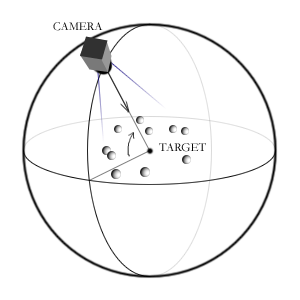
\includegraphics[width=1.75in]{figures/SphereA.png}
	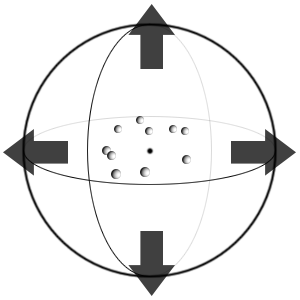
\includegraphics[width=1.75in]{figures/SphereB.png}
	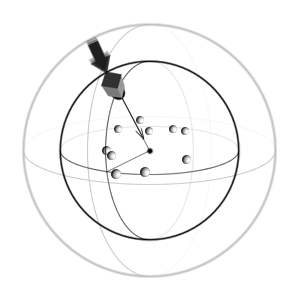
\includegraphics[width=1.75in]{figures/SphereC.png}
	\caption[Mouse input transforms the camera]{Mouse input transforms the camera in different ways.  From left to right, left button (rotation), right button (translation) and left+right buttons (dollying).}
	\label{mouse-input}
\end{figure}
	
\item[Mouse Wheel]
	The mouse wheel moves the camera in and out exactly as the Left + Right drag described above.
	
\item[Mouse clicks]
	The interface uses point and click input for several features, notably particle marking and hiding commands.  Double-clicking a particle will immediately mark it.  Marking functionality is described in detail in the ``Analysis'' section.

\item[Continous Rotation]
	To cause the camera to rotate or drift around the scene, press the ``Page Up'' key.  Each keypress will add velocity to the camera sphere in a clockwise direction.  Pressing ``Page Down'' will add velocity in a counterclockwise direction.  Pressing ``Home'' will stop the camera's movement.

\item[Set Position Menu] 
	Under the Edit menu you will find a ``Set Camera Position'' submenu that allows you to place the camera directly on the X, Y, or Z axes.  You can also engage the ``Follow Particle'' camera mode, which allows you to lock the camera target onto a chosen particle (pressing `f' will also engage this mode).  As the simulation runs, the camera will move with the particle.  To release this mode, select the follow menu command again or press the `f' or escape key.
	
\item[Projection Type]
	The final camera parameter is the ``Toggle Projection'' command.  This command switches between two methods of projecting the 3-D scene onto the 2-D viewing surface.  The default camera view is a perspective projection: the camera's viewing space is a frustrum matching the Z-depths and angle of view set in the ``Scene Options'' dialog.  The camera in this mode is essentially a pinhole camera.  Toggling the mode will switch the view to an orthogonal projection, where parallel lines remain parallel and there are no distance effects.  While the perspective projection matches the eye's perception more closely, the parallel projection is often superior for purposes of analysis.
\end{description}

\subsection{Data Exploration}

\begin{figure}[htb]
	\centering
	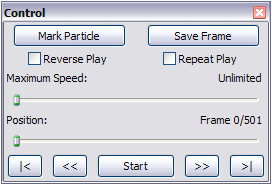
\includegraphics[width=2in]{figures/control-dialog.png}
	\caption[The control dialog for frame navigation]{The control dialog for frame navigation.}
	\label{control-dialog}
\end{figure}

   Once data is loaded, the control dialog (shown in Figure \ref{control-dialog}) is the primary interface to allow a user to easily navigate and playback the entire range of loaded frames.  Along the bottom of the control are five VCR-style playback buttons that enable the user to start and stop the simulation, skip frames one-by-one, and jump to the beginning or end of the simulation.  The Position slider reflects the current frame of the simulation relative to total frames loaded.  By dragging the slider you can skip rapidly to a specific point in the simulation.  The Maximum Speed slider allows the user to control the rate at which frames are rendered during simulation playback.  If the rendering speed is faster than you wish, you can drag the speed slider to the appropriate frames per second setting and the rendering of frames will be restricted to that speed.

   Checking Reverse Play will cause the simulation to play back in reverse, decrementing the frame counter instead of increasing it.  With Repeat Play enabled the simulation will automatically rewind itself and loop back to the beginning (or end) of the loaded frameset.
   
   The ``mark particle'' command prompts the user to select a particle to be marked in the same manner as the Edit $\rightarrow$ Mark Particle command.  Marked particles are highlighted and their paths over time are drawn.  The ``save frame'' command will cause the current rendered frame of the simulation to be saved to a png or avi file.
   
\subsection{Keyboard Input}

  ParticleVis supports a number of keyboard commands for efficient control of the viewpoint and renderer.  Table \ref{keyboard-shortcuts} lists the supported keyboard shortcuts.  Most menus in ParticleVis can also be quickly driven using keystrokes.
  
  Some of the keyboard commands vary slightly from their menu counterparts.  The function keys, in particular, will align the camera to the chosen axis, but unlike the View menu command, will not recenter the view onto the origin.  The arrow and plus/minus keys function in a continous manner, and will spin or dolly the camera as long as they are held down.
  
\begin{table}
\centering
\caption[Keyboard commands in ParticleVis]{Keyboard commands in ParticleVis.}
\label{keyboard-shortcuts}
\begin{scriptsize}
\begin{tabular}[t]{|c r|l|}
\hline \multicolumn{3}{|l|}{Common Keyboard Commands}\\ \hline
	& z & Move to first frame\\
	& x & Move back one frame\\
	& c & Play/Stop\\
	& v & Move forward one frame\\
	& b & Move to last frame\\
	& Ctrl-O & Open statefile\\
	& Ctrl-X & Open descriptor file\\
	& Comma & Cancel file loading\\
	& Escape & Cancel current action\\		
 \hline \multicolumn{3}{|l|}{Marking Commands}\\ \hline
	& p & Mark particle by mouse\\
	& i & Mark particle by ID\\
	& h & Hide particle\\
	& f & Follow particle\\
	& u & Unmark all particles \\
	& Period & Perform visibility selection\\
	& Semicolon & Visibility selection on region\\
	& Slash & Invert current marking selection\\	
\hline \multicolumn{3}{|l|}{Render Commands}\\ \hline
	& a & Auto-set scene options\\
	& 1-5 & Set geometry quality (lowest to highest)\\
	& 6 & Toggle sphere shaders\\
	& l & Toggle lighting\\
	& t, F5 & Toggle texturing\\
	& Ctrl-P & Toggle particles\\
	& Ctrl-V & Toggle translational vectors\\
	& Ctrl-R & Toggle rotational vectors\\
\hline \multicolumn{3}{|l|}{Camera Commands}\\ \hline
	& F2 & Point camera along X axis\\
	& F3 & Point camera along Y axis\\
	& F4 & Point camera along Z axis\\
	& Arrow Keys & Change camera angle \\
	& Plus/Minus & Move closer to or farther from target\\
	& Page Up & Spin camera clockwise \\
	& Page Down & Spin camera counterclockwise \\
	& Home & Halt camera spin \\ \hline	 	
\end{tabular}
\end{scriptsize}
\end{table}

\section{Rendering and Visualization}

A wide variety of methods are available for use in visualizing particle data.  The choice of data to visualize, which elements to emphasize, and the balance between visual fidelity and performance are configurable elements of the visualization.  The primary elements that ParticleVis can visualize are the particles themselves and various forms of vector information.

Particle rendering is usually performed using polygonal approximations of geometry described in an XML descriptor file.  Several levels of quality for the generated geometry are available for selection.  Per-vertex lighting and user-loaded textures can optionally be applied to the surface of rendered polygonal particles.  The set of particles can be rendered in a transparent fashion to give a better view of the entire volume of particles.
When spheres comprise much of the particle data, specialized GLSL shaders that quickly draw pixel-accurate spheres are available.  These high performance shaders are only available if newer (OpenGL 2.0 support) hardware and drivers are present.  Texturing is not currently available when using sphere shaders, but lighting models are applied on a per-pixel basis, allowing high fidelity visualization at any scale.  Finally, a point rendering mode allows for minimal rendering of each particle (as a fixed-size square of pixels).  Using points allows for high rendering performance at the cost of visual fidelity.

A number of vector data sources may also be rendered within ParticleVis.  Data attached to the particles themselves in the form of translational and rotational velocity vectors and normal vectors can be chosen for rendering.  Each type of rendered vector is represented by a line and arrowhead, where each arrowhead is unique to the type of vector rendered.  Data from vector files can also be rendered into the scene.

\subsection{Scene Options}
   Parameters for many of the scene rendering and visualization functions are found in the ``Scene Options'' dialog, which is found under the Edit menu (shown in Figure \ref{scene-dialog}).  Numerical options for the camera, vector rendering, lighting, and other miscellaneous options are found in the scene dialog.
   
\begin{figure}[htb]
	\centering
	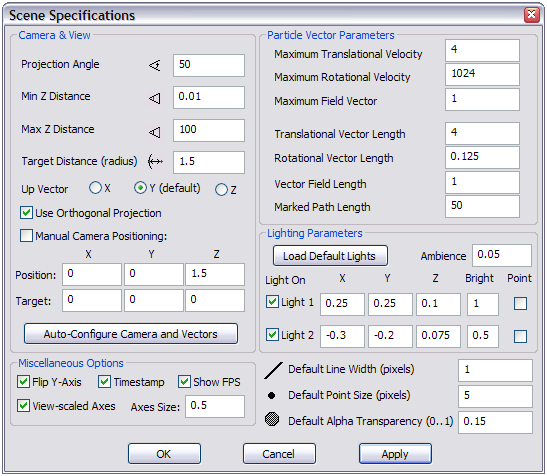
\includegraphics[width=4.5in]{figures/scene-dialog.png}
	\caption[The scene dialog]{The scene dialog.}
	\label{scene-dialog}
\end{figure}

\subsubsection{Camera Parameters}
\begin{description}
\item[Projection Angle]
   The Projection Angle specifies the angle of view that the camera sees when using perspective projection.  A narrower angle affords less distortion and larger particles, whereas a larger angle allows more of the scene to be viewed at once.
\item[Min and Max Z Distance]
The minimum and maximum Z values are the lower and upper limits of distance from the camera within the scene.  Normally, choosing automatic scene settings will set these values (based on the loaded range of positions).  To manually set these values,  choose values such that no particle is beyond the max Z or nearer than the minimum Z (where it would be clipped).  Setting very low values for the minimum Z will allow the camera to be extremely close to viewed particles without clipping, but it may negatively impact the precision of rendering overlapping objects.  The minimum Z must be greater than 0 for proper projection.

\item[Distance/Radius of Rotation]
   This allows the user to manually enter the distance from the camera position to the target.  This affects the radius of the camera's spherical rotation.  See the Camera Control section for more information on camera operation.
   
\item[Orthogonal Projection]
   This option enables an orthogonal projection rather than a perspective projection.  The orthogonal projection is a parallel projection of the scene, and may be more suitable for analysis than the perspective projection.
   
\item[Up Vector]
  If the natural direction of data if different than the default (Y axis), you can change to another axis using these radio buttons.  Since the ParticleVis camera cannot be ``rolled'' away from the up vector, this option can allow more natural viewing of some particle data.

\item[Override Camera Control]
By enabling this override, the user may numerically enter values for the camera position and target.  This allows specification of exact viewpoints reproducibly.  When the override is not enabled, the current position and look-at target are always placed into the dialog.  You may also use the positioner dialog to set force-camera coordinates graphically.  If you wish to see the current position of the camera, note that the position and target fields are updated whenever the scene dialog is opened.
\end{description}

\subsubsection{Vector Parameters}
\begin{description}
\item[Maximum Velocity/Translational Velocity]
  When vectors are drawn they are color-coded by their magnitude.  These two parameters allow you to change the upper value of the mapping, such that the maximum value the user enters is the high end of the color gradient.  The optimal setting will vary between datasets, and should be set such that the highest range of information is mapped into the color gradient.  These parameters also affect Color Scheme mappings in an identical manner.
  
\item[Vector Length]
   Setting this value will scale the length of all vectors.  When this value equals 1.0 the vectors are rendered with length exactly proportional to their values in the raw data, in the same coordinates as particles.  It may be appropriate to rescale the data, so this factor should be set such that the vector length is suitable for visualization.
\item[Marked Path Length]
This parameter determines the length of the pathlines that are drawn behind marked particles.  The value corresponds to the number of frames the path is drawn over.  Setting the parameter to 0 will disable pathlines entirely.  If the pathline length is long, selecting many particles at once may result in poor performance or excessive memory usage.
\end{description}

\subsubsection{Color and Lighting}
\begin{description}
\item[Alpha Transparency]
   When ``Draw Transparent Particles'' is enabled, this value determines the degree of transparency of the particles.  A value of 1 is completely opaque and a value of 0 is completely transparent.  The ultimate appearance of transparent particles is also determined by the blending mode that is being used: additive blending will ``stack up'' the alpha values of overlapping particles, while depth-sorted blending composites underlying layers multiplicatively, leading to a more natural translucency.

\item[Lighting Settings]
ParticleVis uses two directional lights by default.  In this section you may disable or enable the two lights by checking them, and you can adjust the brightness and direction of the lights by editing their vectors.  The light direction is a vector from the specified point to the origin.  The brightness determines the intensity of the light source, from 0 to 1-- higher intensity values can be entered but may appear abnormal.  The positioner dialog can be used to adjust the light direction graphically.

\item[Miscellaneous Options]
Here you can toggle on or off the display of the timestamp in the lower left corner and the display of the frames per second rendered in the lower right.  The FPS counter will be updated once every three seconds.
\end{description}

\subsection{View Commands}
In ParticleVis, the ``View'' menu contains most of the options that control the renderer.   
\begin{description}
\item[Set Geometry Quality]
     Choosing one of the listed options will set all rendered particles to the specified level of geometric detail. By setting lower levels of detail rendering performance can be gained at the expense of visual fidelity. If the program seems to be running too slowly, lower levels of detail should be used.  An option also exists for enabling the use of sphere-specific shaders.  When this option is true, all spheres in the simulation will be rendered using vertex and fragment shaders to quickly render per-pixel accurate spheres.  Subsection \ref{sphereshaders} contains more detail on the various shading styles, which can be selected from the submenu.
\item[Set Color Scheme]
     Allows you to change the color scheme used to color particles.  Whenever color is not specified by the XML descriptor or a loaded color map, the selected scheme will be used to color particles.  You may choose to use white particles, a translational velocity scheme, and a rotational velocity scheme.  The maximum value of translational and rotational velocity, defined in the ``Scene Options'' dialog (Edit menu),  is used to derive the range of values that is mapped onto the color gradient.  A set of common color gradients is provided, and the ``Edit Current Gradient'' will bring up the gradient creator, described in the next section.  The ``Clear Color Maps'' command will clears any color-map data specified from file or XML.
\item[Set Transparency]
     Enabling this option will render some or all of the particles in a partially transparent fashion. Only those particles which are marked via ``Mark Particle'' or have been set as ``noTransparent'' in the XML descriptor are drawn as solid.  By enabling this option and then marking particles it is possible to analyze a subset of the particles in detail while still visualizing the entire particle set.  The rendering mode for transparency is determined by the submenu choice. Additive blending will use a fast method to draw each transparent particle, but it can oversaturate the coloring if the alpha is not carefully set.  Z-sorted alpha blending adds a sorting step which incurs a performance hit, but the rendered particles are drawn in a much more robust manner by using order-dependent alpha blending.  When certain bounding options are enabled (draw under transparency), particles within bounds may always use opaque rendering.
\item[Set Surface Map Properties]
     When a surface map has been loaded into the application, this dialog will allow the tuning of the generated texture coordinates.  The maximum value is set to the maximum recorded surface intensity upon load, but it can be raised or lowered.  The mapping type allows a logarithmic or square root relation to be used in place of the standard linear mapping between scalar intensity and generated texture coordinates.
\item[Use Points]
     Enabling this option will render all the particles as point primitives (squares of pixels) instead of polygonal models.  The rendering performance of sprites is typically must faster than polygonal models, and may be faster than use of sphere shaders.  With very large collections of particles, this option may the only way to allow rendering at acceptable speeds. As sprites, though, the particles cannot be lit or textured, have no orientation, and are much more difficult to distinguish.
\item[Use Textures]
     Enabling this option will add textures to the surface of polygonal particles. Texturing usually has a minimal performance impact and can enhance presentation. A textured surface is useful for discerning particle orientation in particular.
\item[Use Lighting]
Lighting the particles comes at a small performance cost, but it vastly improves the appearance of the particles in most situations.  It is enabled by default.  More options controlling the number and configuration of lights may be found in the ``Scene Options'' dialog (Edit menu).
\item[Use Specular Highlights]
This is a lighting option that calculates a specular highlight on all polygonal surfaces. You may find that this adds visual appeal to the particles, but the option may only be effective at higher polygon counts.  This option will usually incur a small performance cost.
\item[Draw Axes] When enabled, a set of multicolor axes will be drawn on the origin. The axes are scaled to fit in the viewing window, and are labeled by coordinate.
\item[Draw Particles]
    This option controls the rendering of the actual particle objects. Disabling it may be useful when you are rendering some other information that you wish to emphasize, such as vectors.
\item[Draw Normal Vectors]
    When this option is enabled each particle is given a normal vector that corresponds to the up vector in the object coordinates of the individual particle. This is useful to emphasize the orientation of particles where it is otherwise difficult to visualize.
\item[Draw Translational Velocity Vectors]
    When this option is enabled velocity vectors (the first loaded vector) for each particle are drawn. These vectors are color-coded according to magnitude. The length of the vector itself, as well as the mapping of magnitude to color, can be adjusted in the ``Scene Options'' dialog (Edit menu).
\item[Draw Rotational Velocity Vectors]
     When this option is enabled angular velocity vectors (the second loaded vector) for each particle are drawn. The vectors correspond to an axis of rotation and angular velocity about that axis. These vectors are color-coded according to magnitude. The length of the vector itself, as well as the mapping of magnitude to color, can be adjusted in the ``Scene Options'' dialog (Edit menu).
\item[Full-screen Mode]
    This command will size the rendering window such that it fills the entire screen. This is quite useful for presentations. Pressing ``Escape'' or choosing the option again will reset the screen to normal. While in fullscreen mode you cannot see the menu bar, but you can still open it by using shortcut keys (e.g. Alt-V).
\item[Set Window to Size]
    When outputting image files it is often useful to set the window size to a preset value. By choosing one of the submenu sizes you can force the rendering window to a certain dimension. Note that the rendering window will not normally be able to scale beyond the resolution of the monitor. For higher resolution ouput try using the command-line interface.
\item[Show Control Dialog]
     This command will show the control dialog if it has been closed or hidden. 
\end{description}

\subsection{Sphere Shaders}
\label{sphereshaders}

The use of sphere shaders (enabled under the ``View'' menu or pressing `6' ) merits additional discussion.  The sphere shader types available represent a set of shading programs, written in the GLSL language, that efficiently render pixel-accurate spheres.  The different styles of shaders allow the use of various lighting options, image space outlines, rendering styles, and velocity information.

The first two shader types are labled ``Phong Shading'' and ``Phong + Outlines.''  These shading styles are both named for their use of the Blinn-Phong shading model.  This lighting model, which is also used by OpenGL for lighting polygonal models, is used for pixel-accurate lighting, including specular highlights, on the spheres.  Normally only the first light is used for specular reflections (for efficiency), but when the highest quality (``ultra'') is used and the first phong shader is selected, both lights will contribute a specular term.  The primary difference between the two programs is that the outline shader will add a one-pixel black outline to each rendered sphere.  This outline can be useful for distinguishing densely arrayed particles.

The ``Basic Shading'' shader type is a higher performance shader that uses only one light.  Only the diffuse term of the lighting model is used, and no highlights are calculated.  To further increase performance, the depth correction on the spheres has been approximated.  This may lead to the appearance of incorrect intersections between overlapping spheres, but this shader is the fastest type that still retains per-pixel lighting.

The ``Cartoon'' shader type uses a cel-style lighting approach and thick (two pixel) outlines to give a stylized appearance to rendered spheres.  Only the first light is used, and the specular term is included.  As with the ``Phong + Outlines'' style, the outline size is based on screen-space pixels.

The ``Radial Sprite'' shader type is one of the fastest ways to render particles.  Only the outline of the sphere is calculated, and no lighting is used.  When lighting is enabled in the renderer, the distance from the center of the particle is used to attenuate the particle color.  This particle style can be effective when used with the ``Additive Alpha Blending'' transparency option.  When lighting is disabled, a uniformly colored disk is generated.  This shader type is intended for use when high rendering performance or clarity of particle coloring is important.

The ``Perspective-Correct'' shader type employs a per-pixel intersection test that works with complete accuracy when using perspective projections.  For performance reasons, the other shader types assume that a orthogonal (parallel) projection is being used by the camera, and project the silhouette of the sphere as a circle.  In the case of a perspective projection, the actual projected silhouette is in fact an ellipse.  This difference is not generally a critical one, especially with a lower projection angle, as the geometric distortion is usually quite low.  If so desired, though, this shader type allows the exact geometric projection to be used in the shader, albeit at a somewhat high performance cost.  In other respects this shader resembles the ``Basic Shading'' type.

The remaining shading types employ translational velocity information from each particle.  These shaders are designed to function under an orthogonal projection.  The ``Velocity Glyph'' shader will use the translational velocity vector of the particle to render an arrow glyph that points in the screen-space direction of the particle's motion.  This glyph is inscribed onto the surface of the sphere, and does not take the vector magnitude into account.  The resulting effect is similar to a hedgehog-style vector plot.  Enabling color mapping can help to elucidate the magnitude of the vectors.

To incorporate the effect of vector magnitude directly into the arrow glyph, the ``Velocity Glyph (Scaled)'' shader style can also be used.  This shader type uses the translational velocity vector length parameter (set in the ``Scene Options'' dialog) to scale the thickness of the glyph according to its magnitude.  By setting the vector length to an appropriate ratio, a suitable range of thicknesses can be achieved.  The vector length scaler (see \ref{misc-tools}) is a good tool for accomplishing this.

The ``Velocity Motion Blur'' shader style uses the translational velocity to create a camera motion blur effect on moving particles.  This shader blurs the particles in the screen-space direction of their translational velocity vector, by a factor calculated from the translational velocity length parameter and the vector magnitude (as in the previous shader type).  This effect has a high performance cost, but can be useful for presentational purposes.  To accomplish proper composition, Z-sorted alpha blending is used when this shader type is enabled.

\subsection{Volumetric Rendering}

ParticleVis provides the ability to render static volumetric data into the visualization.  By loading a volume file with the corresponding command under the ``Analysis'' menu, a file of raw volume data can be rendered.  To enable and disable the use of the loaded volume data, use the ``Enable Volumetric Rendering'' command under the ``Analysis'' menu.

The rendering of volume data can be adjusted by choosing the ``Volumetric Rendering Options'' command under ``Analysis.''  If no volume data is currently loaded, choosing ``Use Dummy Data'' will generate a spherical volume for testing purposes.  Each X-Y slice can be normalized individually, for both coloring and alpha intensity, as opposed to globally by checking the appropriate option.  The volume slices will use alpha-based blending by default, but an additive blending mode can also be enabled.  Each time the volume rendering options dialog is used, the current gradient will be re-applied to the loaded volume data, updating the volume's coloring.

The ``Max Alpha'' of the volume determines the transparency range the slices are mapped to, from zero to 255.  Raising or lowering it will change the overall transparency of the volume.  ``Slice size'' is the measure of the width of the set of slices, and should be set to match the volume's scale, so that no clipping occurs during rendering.  The number of slices is the total number of generated slices.  Increasing the slice count will result in a higher fidelity rendering, but will also increase load in terms of graphical fill rate.

The volume can be transformed using the origin, rotation, and scale fields in the options dialog.  The origin is the centerpoint of the volume in world coordinates.  The rotation fields describe a series of rotations in degrees, in order X-Y-Z, which can reorient the volume as needed.  The scale fields allow rescaling of the volume in each axial direction.  The volume will first be scaled, then rotated, and then translated.

The analysis menu also contains a ``Create Density Volume'' command that can generate a simple spatial view of average density based on the loaded particle state data.  Once the state data is loaded, this command can be executed by inputting a resolution for the cubic size of the volume.  A large resolution will produce cubic cells of small size, and vice versa.  The loaded state data will then be traversed and the presence of particles in each spatial cell will be compiled and averaged over all frames.  For each frame, every particle that is present in a cell will increment the cell's density measure by one.  The current gradient is then used to color each cell based on its normalized density.

\subsection{Miscellaneous Tools}
\label{misc-tools}

  Several other functions within ParticleVis allow configuration of rendering and visualization: the gradient editor, the positioning tool, and the vector length scaling tool.
  
  The gradient editor displays the current ramp of color that is used for certain coloring schemes for both particles and vectorlines.  The gradient is specified by a series of color knots.  Color is linearly interpolated between the knots to produce a smooth ramp.  Changing the gradient is accomplished entirely with mouse input.  Clicking and dragging a knot updates its position.  New knots with the current color can be added, and existing knots can be deleted.  The ``number of generated colors'' field controls the fidelity of the generated gradient: if only a small number of discrete colors is desired, set this field to a low value.  Gradients can be also be saved and loaded to and from files.
  
  The positioning tool is found under Edit $\rightarrow$ Position Camera/Lights.  This tool allows mouse-based positioning of light sources and the camera.  To point the camera into a specific position, select the modal toggle to place a camera position and target into the scene, then press the ``Force Camera Position'' button.  The viewpoint will be locked into this position until the escape key is pressed or the option is disabled under ``Scene Options.''  A camera cone showing the range of the potential viewpoint can be drawn during this process.  Selecting the light toggles allows you to move the lights around the scene interactively.  Depending on the lighting options, the rendered position may be the light's direction or point position.  Pressing escape will exit this positioning mode as well.
  
  The vector length scaler, found under the ``View'' menu, allows interactive adjustment of vector glyph length.  Each vectorline type can be scaled by dragging or clicking its corresponding scaler bar.  The scale values are exactly as they are found in the ``Scene Options'' dialog.  When you have finished scaling, press escape or close the tool to return to normal input.

\section{Analysis}
	A series of tools are provided in ParticleVis that are useful for simple analysis.  The ability to mark particles by mouse selection, region, or ID is provided.  Each marked particle is given a highlighted color in the visualization, a pathline of configurable length, and a line of text in the console that reports current position and velocity.  More advanced marking operations are provided in the visibility selection tool.  A facility for bounding or clipping out spatial regions is also provided.  It is also possible to generate windowed graphs that display individual particle state information over time.
	
	The aim of all these features is to allow more specific queries into the loaded data.  However, there are few features inside ParticleVis proper that are able to generate derived data from the particle states.  Instead, file formats such as color and surface maps exist to allow arbitrarily generated data to be loaded onto the visualized particles.  Subgraphs of scalar value per time step (comma separated value files) can also be loaded and displayed in subwindows.  If the existing coloring options are insufficient, color maps allow the loading of color information for any or all of the particles at each timestep.  Surface maps allow even more control, as they specify an array of scalars that are mapped onto each rendered particle.  The vector file format can also be used to overlay additional data onto the loaded state, and volume files can be used to provide additional (static) spatial data.
		
\subsection{Marking Particles}

	Each particle in the visualization possesses a marking state that indicates if the particle should be highlighted and tracked.  Particles may also be hidden, or flagged to indicate that they should not be drawn transparently.  Marking can be done using the mouse, ID input, or options in XML files.  The edit menu contains the marking commands: ``Mark particles for Tracking'' (`p' key), ''Mark particle to hide'' (`h' key), and ``Mark particle to follow'' use mouse input.  Following a particle will lock the camera target to the position of the marked particle until the command is repeated or escape is pressed.   ``Mark particle by ID'' (`i' key) uses a numerical ID that corresponds to the ordering of particles in the statefile, starting from zero.  The ``Unmark all Particles'' or the `u' key will clear all marking states.
	
	More complex marking operations can be performed using the visibility selector, found under the edit menu.  Most of the visibility functionality requires a graphics card that supports hardware occlusion queries.  The visibility selector allows all currently visible particles or all particles within a selected region to be marked.  Optionally, the inverse of the selection (hidden particles) can be used by selecting the ``Select Occluded Particles'' radio button.  The marking action that is applied is determined by the selection of checkboxes in the selector dialog.  Pressing period or ``Select Entire View'' will use the entire rendered viewpoint for selection, while pressing semicolon or ``Select Region'' allows a rectangular area to be drawn out for selection.  The ``Invert Marking'' command (forward slash) will invert the mark state of all particles: currently unmarked particles will be marked, and currently marked particles will be unmarked.  When all particles are unselected this can be used to quickly mark the whole set.  ``Reset States'' will clear all marking information from particles.

\subsection{Bounding Particles}

	The bounding options in ParticleVis allow you to restrict particle rendering to a certain spatial range.  Opening the bounds dialog under the edit menu allows the configuration of a range of allowed X, Y, or Z positions.  Enabling one or more of the checks will engage the range check.  This can also be thought of as a series of axis aligned clipping planes.  
	
	When transparency is enabled, you can render both bounded and unbounded particles by selectively applying transparency to particles outside the range instead of hiding them.  The ``draw bounded particles under transparency'' option controls this feature.